\documentclass[xcolor ={table,usenames,dvipsnames}]{beamer}
\usepackage[italian]{babel}
\usepackage{listings}
\usepackage{txfonts}
\PassOptionsToPackage{dvipsnames}{xcolor}
\title{Multivariate Analysis and Statistical Learning \\ Implementazione PC Algorithm}

\author{Authors: Alex Foglia, Tommaso Puccetti}
\institute{Universit\`a  degli Studi di Firenze}
\date{21/12/2018}
%\usepackage{sansmathaccent}
\usetheme{Berlin} 
\useinnertheme{rounded}
\useoutertheme{miniframes} 
\setbeamercovered{dynamic}
 
\theoremstyle{definition}
\newtheorem{definizione}{Definizione}

\begin{document}
	
	\begin{frame}
		\maketitle
	\end{frame}

	\begin{frame}
		\frametitle{Accenni teorici (1)}
		\begin{itemize}
			\item Le reti Bayesiane possono essere rappresentate attraverso l'utilizzo di un grafo aciclico diretto, o \textbf{DAG}.\\
			\item Un DAG è un grafo diretto in cui non compaiono cicli, dove per ciclo si intende un qualunque cammino finito che, a partire da un nodo iniziale $v$ termini in $v$.
		\end{itemize}
	\end{frame}

	\begin{frame}
		\frametitle{Accenni teorici (2)}
		Sia $G = (V,E)$ un DAG su un insieme finito $X = \{X_v \forall v \in V\}$ di variabili casuali, allora:
		$$
		\forall u,v \in V \;non\;adiacenti\;| v \in nd(u) \Rightarrow u \Perp v | nd(u) - v
		$$
		Dove $nd(u)$ è l'insieme dei nodi \emph{non discendenti} di u, ossia tutti quei nodi $u'$ per cui non esiste un cammino da $u$ a $u'$.\\
	\end{frame}

	\begin{frame}
		\frametitle{PC-Algorithm}
		Dato un insieme di variabili con distribuzione di probabilità congiunta gaussiana, è possibile imparare il DAG sottostante al campione osservato attraverso l'utilizzo del \textbf{PC-Algorithm}.\\
		Esso è composto da due sotto-funzioni che risolvono due diversi problemi:
		\begin{enumerate}
			\item La costruzione dello scheletro (o grafo morale)
			\item La costruzione del DAG a partire da un dato scheletro
		\end{enumerate}
	\end{frame}

	\begin{frame}
		\frametitle{Pseudocodice: generazione dello scheletro}
		\begin{figure}[h!]
			\centering
			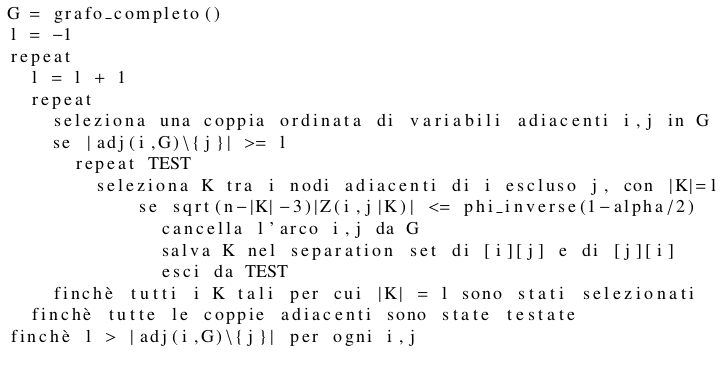
\includegraphics[scale=0.53]{img/pcalg.PNG}
			\label{Interfacce di un CS}
		\end{figure}
	\end{frame}

	\begin{frame}
		\frametitle{Pseudocodice: costruzione del DAG}
		\begin{figure}[h!]
			\centering
			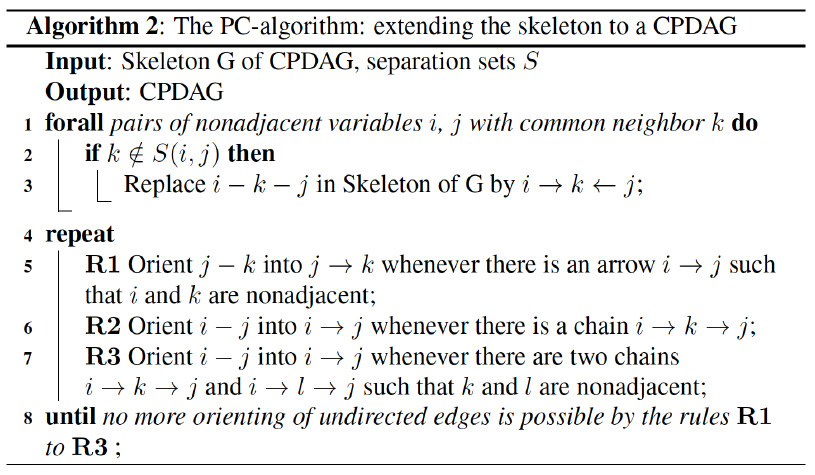
\includegraphics[scale=0.5]{img/pcalg2.PNG}
			\label{Interfacce di un CS}
		\end{figure}
	\end{frame}
	
\end{document}